\documentclass{article}

\usepackage[utf8]{inputenc}
\usepackage[spanish]{babel}
\usepackage[a4paper,top=2cm,bottom=2cm,left=3cm,right=3cm,marginparwidth=1.75cm]{geometry}
\usepackage{amsmath}
\usepackage{graphicx}
\graphicspath{{imagenes/}}
\usepackage{float}
\usepackage{caption}
\usepackage[colorlinks=true, allcolors=blue]{hyperref}
\usepackage{lipsum}
\usepackage{setspace}
\usepackage{tikz}
\usepackage{xcolor}
\definecolor{guinda}{rgb}{0.28, 0.02, 0.03}
\usepackage[left=2.5cm, right=2.5cm,top=2.5cm,bottom=2.5cm]{geometry}
\usepackage[colorlinks=true, allcolors=blue]{hyperref}

\title{\textbf{%
    Universidad Nacional de San Agustín \\
    Maestría en Ciencias de la Computación \\
    \large Análisis del Problema del Agente Viajero}}
\author{Abel E. Borit Guitton, Luis A. Borit Guitton, Betzy J. Yarín Ramírez}
% \date{\today}
\date{17 de agosto de 2023}

\begin{document}
\begin{titlepage}
    \begin{center}
    \begin{tikzpicture}[remember picture, overlay]  
        \definecolor{guinda}{rgb}{0.28, 0.02, 0.03}
        \draw[guinda, line width=3pt, rounded corners=10pt]
        ([shift={(2cm,-2cm)}]current page.north west)
        rectangle
        ([shift={(-2cm,2cm)}]current page.south east);
    \end{tikzpicture}

    \centering
            {\huge\textbf{Universidad Nacional de San Agustín}}\\
            \vspace{6mm}
            \begin{figure}[h]
                \centering           
                \includegraphics[height=6cm]{Escudo_UNSA.png}
            \end{figure}
            \vspace{6mm}
            {\LARGE\textbf{Escuela Profesional Ciencias de la Computación}}\\
            \vspace{5mm}
            {\LARGE\textbf{Maestría en Ciencias de la Computación}}
            \vspace{6mm}\\
            {\Large Algoritmos y Estructura de Datos}
            \vspace{5mm}\\
            \textcolor{guinda}{\rule{\linewidth}{0.75mm}}\\
            \vspace{2mm}
            \begin{spacing}{1.5}
            {\LARGE\textsc{Análisis del Problema del Agente Viajero} }
            \end{spacing}
            \textcolor{guinda}{\rule{\linewidth}{0.75mm}}\\
            \vspace{1cm}
            \Large\textbf{Docente: Ph.D.(c) Vicente Machaca Arceda}\\
            \vspace{1.3cm} 
            \Large\textbf{Participantes:}\\    
            \vspace{3mm}
            \Large Abel E. Borit Guitton \\
            \Large Luis A. Borit Guitton \\
            \Large Betzy J. Yarín Ramírez \\
            \vspace{2cm}
            \Huge\textbf{2023}

    \end{center}
\end{titlepage}
\maketitle
\tableofcontents
\clearpage

\section{INTRODUCCION}
\subsection{Introducción a Teoria de Grafos}
En matemáticas, la teoría de grafos [1] es el estudio de los gráficos, que son estructuras matemáticas utilizadas para modelar relaciones por pares entre objetos. Un grafo en este contexto se compone de vértices (también llamados nodos o puntos) que están conectados por aristas (también llamados enlaces o líneas). Se hace una distinción entre grafos no dirigidos, donde las aristas unen dos vértices simétricamente, y gráficos dirigidos, donde las aristas unen dos vértices asimétricamente. Los gráficos son uno de los principales objetos de estudio de las matemáticas discretas.

\subsection{Introducción al problema del agente viajero}
El problema del agente viajero [2](Traveling Salesman Problem, TSP) es un problema de optimización combinatoria (se trata de un problema de optimización que involucra una cantidad finita o numerable de soluciones posibles) en el campo de la teoría de la computación y la investigación de operaciones. 

Se trata de encontrar la ruta más corta posible que permita a un agente visitar un conjunto dado de ciudades y regresar a la ciudad de origen, pasando por cada ciudad exactamente una vez.

\subsection{Introducción a heurísticas}
Cuando un algoritmo usa una heurística[6], ya no necesita buscar de manera exhaustiva todas las soluciones posibles, y por tanto puede encontrar soluciones aproximadas mas rápido. Una heuristica es un atajo que sacrifica exactitud por rapidez.

\subsection{Introducción a metaheurísticas}
Los metaheurísticos son métodos aproximados diseñados para resolver problemas de optimización combinatoria, en los que los heurísticos clásicos no son efectivos.

% *****************************************************************
\section{PROBLEMA DEL AGENTE VIAJERO}
    \begin{enumerate}
        \item El objetivo es encontrar una forma de hacer su viaje más eficiente [2] (en términos de la distancia total recorrida o del costo total).       
        
        \item El problema se puede modelar mediante un grafo etiquetado (las aristas tienen distancias o costos asociados a ellas), en el cual buscamos el ciclo hamiltoneano más eficiente. En la Figura 1, se muestra esta representación. 
        
        \item Para un grafo de n vértices, tenemos (n - 1)! posibles ciclos hamiltonianos.
    \end{enumerate}  

Para resolver el problema del agente viajero, se utilizaron, como prueba y estructura para resolver el problema, los siguientes datos:
    
    \begin{enumerate}
        \item Nodo Grand Rapids:       
            \begin{enumerate}
                \item Desde Grand Rapids a Grand Rapids es 0       
                \item Desde Grand Rapids a Saginaw es 113      
                \item Desde Grand Rapids a Detroit es 147      
                \item Desde Grand Rapids a Toledo es 167       
                \item Desde Grand Rapids a Kalamazoo es 56     
            \end{enumerate}

        \item Nodo Saginaw:     
            \begin{enumerate}
                \item Desde Saginaw a Grand Rapids es 113      
                \item Desde Saginaw a Saginaw es 0      
                \item Desde Saginaw a Detroit es 98      
                \item Desde Saginaw a Toledo es 142       
                \item Desde Saginaw a Kalamazoo es 137 \\     
            \end{enumerate}

        \item Nodo Detroit:      
            \begin{enumerate}
                \item Desde Detroit a Grand Rapids es 147      
                \item Desde Detroit a Saginaw es 98      
                \item Desde Detroit a Detroit es 0     
                \item Desde Detroit a Toledo es 58       
                \item Desde Detroit a Kalamazoo es 135     
            \end{enumerate}

        \item Nodo Toledo:      
            \begin{enumerate}
                \item Desde Toledo a Grand Rapids es 167       
                \item Desde Toledo a Saginaw es 142     
                \item Desde Toledo a Detroit es 58    
                \item Desde Toledo a Toledo es 0       
                \item Desde Toledo a Kalamazoo es 133
            \end{enumerate}

        \item Nodo Kalamazoo:      
            \begin{enumerate}
                \item Desde Kalamazoo a Grand Rapids es 56      
                \item Desde Kalamazoo a Saginaw es 137      
                \item Desde Kalamazoo a Detroit es 135    
                \item Desde Kalamazoo a Toledo es 133      
                \item Desde Kalamazoo a Kalamazoo es 0    
            \end{enumerate}

    \end{enumerate}

\begin{table}[H]
  \centering
  \begin{tabular}{||c c c c c c||} 
    \hline
    \textbf{} & \textbf{Grand Rapids} & \textbf{Saginaw} & \textbf{Detroit} & \textbf{Toledo} & \textbf{Kalamazoo} \\ [0.5ex] 
    \hline\hline
    Grand Rapids    &  0     &  113  &  147  &  167  &  56   \\ [0.5ex]
    Saginaw         &  113   &  0    &  98   &  142  &  137  \\ [0.5ex]
    Detroit         &  147   &  98   &  0    &  58   &  135  \\ [0.5ex]
    Toledo          &  167   &  142  &  58   &  0    &  133  \\ [0.5ex]
    Kalamazoo       &  56    &  137  &  135  &  133  &  0    \\ [0.5ex]
    \hline
  \end{tabular}
  \caption{Problema del Agente Viajero (Matriz)}
  \label{table:AgenteViajeroMatriz}
\end{table} 

\begin{figure}[H]
    \centering
    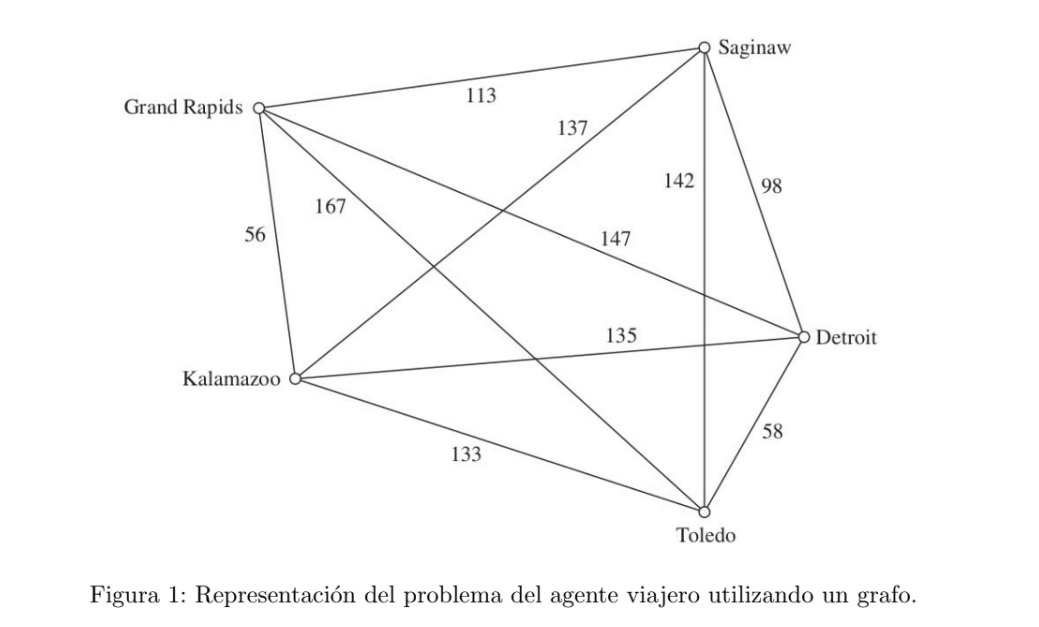
\includegraphics[width=0.9\textwidth]{imagenes/ProblemaAgenteViajero.jpg}
    \caption{\label{fig:problemaAgenteViajero}Problema del Agente Viajero}
\end{figure}

% *****************************************************************

\section{ALGORITMOS}
\subsection{ALGORITMO DEL ÁRBOL DE EXPANSIÓN MÍNIMA (MINIMUM SPANNING TREE, MST)}
Se construye un árbol de expansión mínima [3] a partir de las ciudades y luego se recorre para formar una ruta. El algoritmo encuentra un subconjunto de aristas que forman un árbol con todos los vértices, donde el peso total de todas las aristas en el árbol es el mínimo posible.

Este algoritmo es ampliamente utilizado en teoría de grafos y optimización combinatoria para encontrar un subconjunto de aristas de un grafo conexo que conecta todos los vértices y tiene un peso total mínimo.

El Algoritmo del Árbol de Expansión Mínima es mejor para grandes cantidades de datos:

    \begin{enumerate}
        \item \textbf{Optimización garantizada:} El MST garantiza una solución óptima para el problema del Agente Viajero si el gráfico (grafo completo con pesos en este caso) cumple con la propiedad del triángulo. Esta propiedad establece que para cualquier conjunto de tres ciudades, el camino más largo entre dos de ellas no es mayor que la suma de los otros dos caminos. Esto asegura que el MST proporcionará una solución cercana a la óptima para TSP.
        
        \item \textbf{Enfoque heurístico:} Aunque no es necesariamente la solución más óptima en todos los casos, el MST se comporta bien en la práctica para muchas instancias de TSP, especialmente para casos con un gran número de ciudades.
        
        \item \textbf{Escalabilidad:} A medida que el número de ciudades aumenta, la diferencia en la eficiencia entre los algoritmos se hace más evidente. El MST es más escalable en términos de tiempo de ejecución.
    \end{enumerate}

\begin{figure}[H]
    \centering
    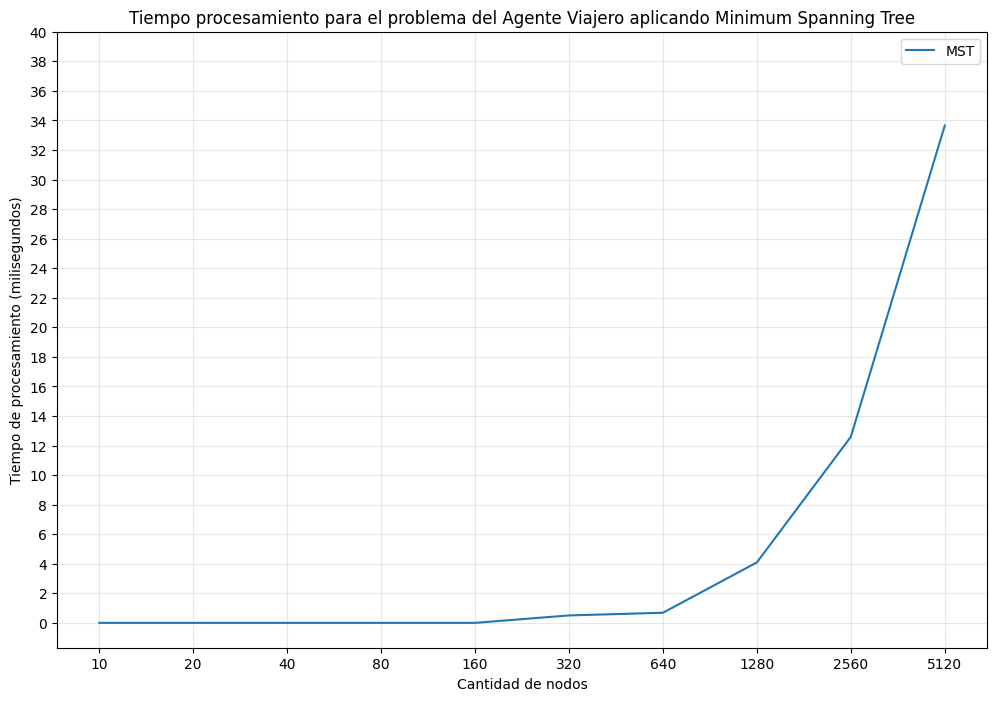
\includegraphics[width=0.88\textwidth]{imagenes/GraphicMST.png}
    \caption{\label{fig:GraphicMST}Tiempo procesamiento para el problema del Agente Viajero aplicando Minimum Spanning Tree}
\end{figure}

\subsection{ALGORITMO GENÉTICO}
Los algoritmos genéticos [4] son técnicas de optimización y búsqueda inspiradas en la evolución biológica. Utilizan operadores como selección, cruza y mutación para evolucionar una población de soluciones candidatas en busca de soluciones óptimas o cercanas a óptimas para problemas complejos.

    \begin{enumerate}
        \item \textbf{Aplicación del algoritmo:} Para el problema del viajante en teoría de grafos, los algoritmos genéticos generan rutas entre ciudades representadas por cromosomas, donde cada cromosoma es una permutación de las ciudades. La función de aptitud evalúa la distancia total de cada ruta. La selección de padres, cruza y mutación simulan procesos de selección natural y reproducción, creando nuevas rutas que tienden a mejorar la distancia total con el tiempo. Esto permite encontrar soluciones que buscan minimizar la distancia recorrida en el recorrido del viajante a través de todas las ciudades.
    \end{enumerate}

\begin{figure}[H]
    \centering
    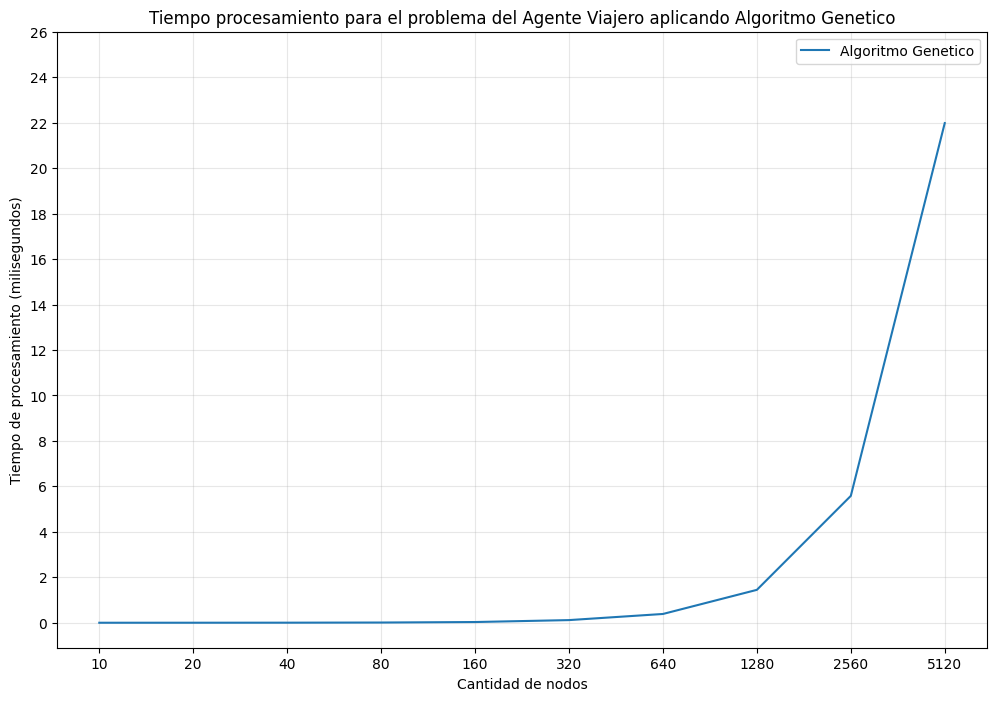
\includegraphics[width=0.88\textwidth]{imagenes/GraphGeneticAlgorithm.png}
    \caption{\label{fig:GraphGeneticAlgorithm}Tiempo procesamiento para el problema del Agente Viajero aplicando Algoritmo Genéticos}
\end{figure}


\subsection{ALGORITMO DE BÚSQUEDA LOCAL}
Es una técnica heurística y este algoritmo [5] es utilizado para resolver problemas de optimización, como planificación de rutas, diseño de redes, programación de horarios, etc.

Explora el espacio de soluciones vecinas a la solución actual en busca de mejoras significativas. Obvia la lista de todas las soluciones generadas, solo centra su atención en mejorar la solución actual.

Pero puede quedar atrapado en mínimos locales, es decir podría no llegar a la solución óptima global del problema, y esta es una considerable limitante.

    \begin{enumerate}
        \item \textbf{Inicialización:} Empieza en un punto de partida aleatorio o determinado.
        
        \item \textbf{Evaluación de vecindad:} Crea una vecindad de soluciones, las rutas tienen una cierta diferencia de la solución actual, ejemplo intercambia dos ciudades en la ruta para crear una solución vecina.
        
        \item \textbf{Evaluación de la función objetivo:} Calcula la distancia total de la ruta para cada solución en la vecindad generada. 
        
        \item \textbf{Selección de la mejor solución vecina:} Escoge la solución con la menor distancia. Compara la distancia total de la mejor solución vecina con la solución actual. Si la última es mejor, realiza un intercambio, reemplaza la solución actual por la solución vecina. 
        
        \item \textbf{Criterio de parada:} Repite los pasos 2, 3 y 4 hasta que alcance un criterio de determinación, es decir ya no encuentre mejoras significativas en un número determinado de iteraciones. Es allí donde el algoritmo se detiene.
    \end{enumerate}

\begin{figure}[H]
    \centering
    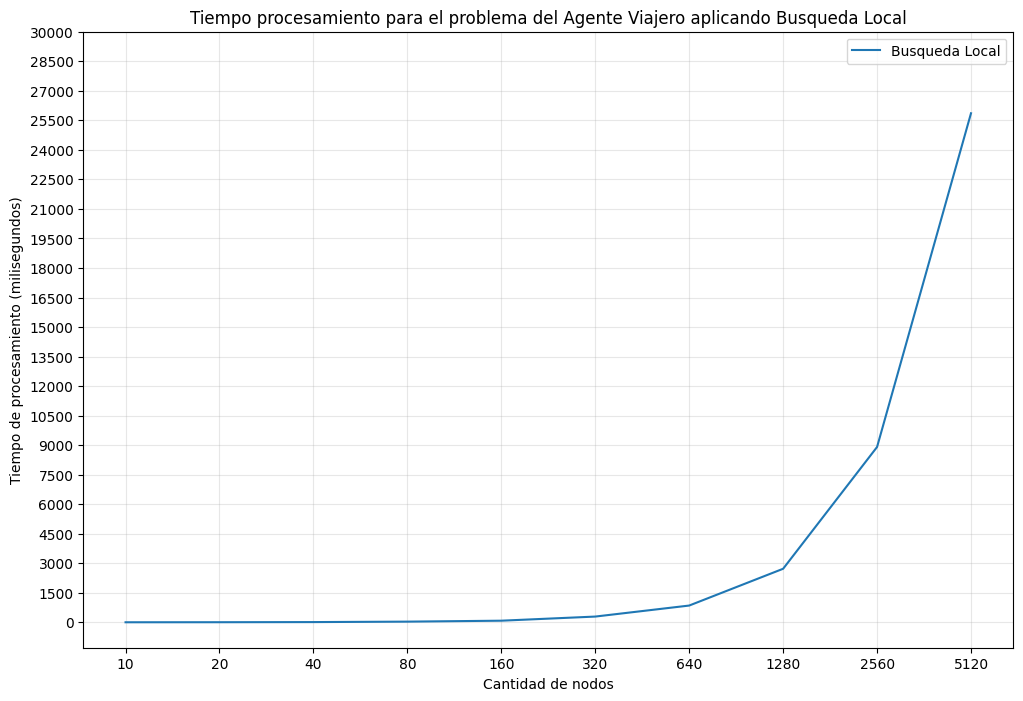
\includegraphics[width=0.88\textwidth]{imagenes/GraphicBusquedaLocal.png}
    \caption{\label{fig:GraphicBusquedaLocal}Tiempo procesamiento para el problema del Agente Viajero aplicando Búsquedas Locales}
\end{figure}


% *****************************************************************

\section{IMPLEMENTACION}
En el siguiente enlace \href{https://github.com/abelborit/computer-science-master/tree/main/MCC-01_algorithms-and-data-structures/graphs-analysis}{Repositorio GitHub} se podrá visualizar toda la implementación realizada. Cuenta con un file system estructurado para cada algoritmo usado, archivos externos de donde se tomarán los datos de entrada para los algoritmos (cabe mencionar que los archivos se tendrán que generar corriendo los archivos de python ya que GitHub no permite más de 100MB), una carpeta donde está el código usado para realizar gráficas con el Matplotlib como sus gráficas correspondientes y también un archivo README.md propio del proyecto y repositorio.

\section{RESULTADOS}
\subsection{COMPARATIVA DEL TIEMPO DE EJECUCIÓN EN GO (milisegundos)}
\begin{enumerate}
    \item \textbf{Algoritmo MST:} Minimum Spanning Tree (ejecutado en laptop con tarjeta grafica y RAM de 16GB)
    \item \textbf{Algoritmo Genetico:} Algoritmo Genetico (ejecutado en una Macbook AIR M1 2020)
    \item \textbf{Algoritmo MLS:} Minimum Local Search (ejecutado en una PC)
\end{enumerate}


\begin{table}[H]
    \centering
    \begin{tabular}{||c c c c||} 
      \hline
      \textbf{Cantidad de Nodos} & \textbf{Algoritmo MST} & \textbf{Algoritmo Genetico} & \textbf{Algoritmo MLS} \\ [0.5ex] 
      \hline\hline
      10    &  0.0000   &  0.001149  &  4.2656      \\ [0.5ex]
      20    &  0.0000   &  0.001898  &  7.1241      \\ [0.5ex]
      40    &  0.0000   &  0.003752  &  13.8356     \\ [0.5ex]
      80    &  0.0000   &  0.010151  &  36.5711     \\ [0.5ex]
      160   &  0.0000   &  0.032446  &  84.2718     \\ [0.5ex]
      320   &  0.5024   &  0.117269  &  293.8134    \\ [0.5ex]
      640   &  0.6837   &  0.386897  &  853.6143    \\ [0.5ex]
      1280  &  4.0896   &  1.447995  &  2722.0933   \\ [0.5ex]
      2560  &  12.5886  &  5.582167  &  8907.4015   \\ [0.5ex]
      5120  &  33.6501  &  21.98101  &  25858.1051  \\ [0.5ex]
      \hline
    \end{tabular}
    \caption{Comparativa de Tiempo de ejecución (milisegundos)}
    \label{table:tiempoEjecucion}
\end{table} 

% *****************************************************************

\section{CONCLUSIONES}
\subsection{ALGORITMO DEL ÁRBOL DE EXPANSIÓN MÍNIMA:}
\begin{enumerate}
  \item El algoritmo está diseñado para minimizar la distancia total recorrida, lo que es crucial en escenarios donde se busca ahorrar tiempo, recursos y costos de transporte. Proporciona una solución eficiente para encontrar la ruta más corta.
  \item Al encontrar la ruta más corta, se minimiza el consumo de recursos como combustible, tiempo y energía. Esto es esencial para lograr operaciones más eficientes y sostenibles en diversas áreas, también se reducen los costos asociados con el transporte y la logística, lo que impacta positivamente en la rentabilidad de las operaciones.
  \item La automatización de la planificación de rutas mediante este algoritmo ayuda a optimizar tareas que de otra manera requerirían mucho tiempo y esfuerzo humano. Además, garantiza una planificación coherente y precisa.
  \item En resumen, la aplicación del algoritmo del Agente Viajero basado en el Minimum Spanning Tree representa una solución valiosa para optimizar la planificación de rutas y la asignación de recursos en una variedad de contextos. Su capacidad para encontrar rutas eficientes y minimizar distancias hace que sea una herramienta esencial para mejorar la eficiencia y reducir costos en diversas industrias.
\end{enumerate}

\subsection{ALGORITMO GENÉTICO:}
\begin{enumerate}
  \item En conclusión, los algoritmos genéticos son poderosas técnicas de optimización y búsqueda que encuentran inspiración en el proceso de evolución biológica. Estos algoritmos se aplican a problemas complejos con el objetivo de encontrar soluciones óptimas o cercanas a óptimas. En el ámbito de la teoría de grafos, los algoritmos genéticos ofrecen una perspectiva innovadora para abordar el problema del viajante.
  \item En el contexto del problema del viajante en teoría de grafos, los algoritmos genéticos se presentan como una herramienta valiosa. Mediante la representación de rutas entre ciudades como cromosomas y la aplicación de operadores como selección, cruza y mutación, se busca encontrar rutas que minimicen la distancia total recorrida. La función de aptitud juega un papel crucial al evaluar y comparar la eficacia de diferentes rutas.
  \item La analogía con la selección natural y la reproducción en biología permite que los algoritmos genéticos generen nuevas rutas que mejoran progresivamente la distancia total recorrida. Esta adaptación gradual a lo largo de múltiples generaciones conduce a la convergencia hacia soluciones más óptimas. En resumen, los algoritmos genéticos proporcionan una estrategia efectiva para abordar problemas complejos en teoría de grafos, como el problema del viajante, al combinar conceptos biológicos con técnicas de optimización computacional.
\end{enumerate}

\subsection{ALGORITMO DE BÚSQUEDA LOCAL:}
\begin{enumerate}
  \item En el algoritmo de Búsqueda Local, la calidad de los resultados obtenidos tiene una fuerte dependencia con la elección de la solución inicial y la estrategia de generación de vecindad.
  \item Para superar la limitante del algoritmo de búsqueda, se pueden experimentar con variaciones del algoritmo, como la búsqueda local iterada o combinar con otras técnicas de optimización.
  \item El algoritmo de búsqueda local es eficiente en términos de tiempo de ejecución, porque su objetivo no es examinar todas las soluciones posibles. Es muy útil para resolver problemas de la vida real cuando se tiene limitación de recursos y se requiere una solución aceptable en un tiempo razonable.
\end{enumerate}

Es importante tener en cuenta que los resultados de tiempo de ejecución pueden variar según el hardware y el entorno de ejecución utilizado para las pruebas (así como se demostró en las implementaciones del presente análisis). Se recomienda realizar pruebas adicionales y comparaciones en un contexto específico antes de tomar decisiones finales sobre qué algoritmo y lenguaje de programación utilizar en un proyecto real.

\clearpage
\begin{thebibliography}{widest entry} 
  \bibitem[1]{} Bender \& Williamson 2010, p. 148.
  \bibitem[2]{} Behzad, Arash; Modarres, Mohammad (2002)
  \bibitem[3]{} Bernard Chazelle, 1999
  \bibitem[4]{}  D. E. Goldberg. Addison-Wesley Longman Publishing Co., Inc., Boston, MA, USA. 1989. 
  \bibitem[5]{} D. Schuurmans and F. Southey. Local search characteristics of in- complete SAT procedures
  \bibitem[6]{} Moustakas, Clark (1990). Heuristic Research: Design, Methodology and Applications
 \end{thebibliography}

\end{document}